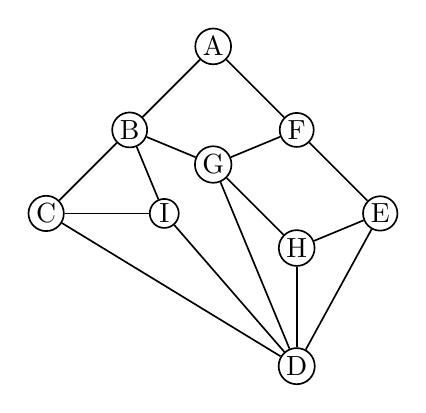
\begin{tikzpicture}[scale=0.25,node distance=1.5cm,semithick,inner sep=1pt,bend angle=45]
%\draw[help lines] (-3,-3) grid (3,0);
\node[circle,draw]   (v1)                     {\tf A};
\node[circle,draw]   (v2) [below left  of=v1] {\tf B};
\node[circle,draw]   (v3) [below right of=v1] {\tf F};
\node[circle,draw]   (v4) [below left  of=v2] {\tf C};
\node[circle,draw]   (v5) [below       of=v1] {\tf G};
\node[circle,draw]   (v6) [below right of=v3] {\tf E};
\node[circle,draw]   (v7) [below right of=v5] {\tf H};
\node[circle,draw]   (v8) [right       of=v4] {\tf I};
\node[circle,draw]   (v9) [below       of=v7] {\tf D};

\path
(v1) edge node{} (v2)
     edge node{} (v3)
(v2) edge node{} (v4)
     edge node{} (v5)
     edge node{} (v8)
(v3) edge node{} (v5)
     edge node{} (v6)
(v4) edge node{} (v8)
     edge node{} (v9)
(v5) edge node{} (v7)
     edge node{} (v9)
(v6) edge node{} (v7)
     edge node{} (v9)
(v7) edge node{} (v9)
(v8) edge node{} (v9);                     
\end{tikzpicture}
